%  A simple AAU report template.
%  2015-05-08 v. 1.2.0
%  Copyright 2010-2015 by Jesper Kjær Nielsen <jkn@es.aau.dk>
%
%  This is free software: you can redistribute it and/or modify
%  it under the terms of the GNU General Public License as published by
%  the Free Software Foundation, either version 3 of the License, or
%  (at your option) any later version.
%
%  This is distributed in the hope that it will be useful,
%  but WITHOUT ANY WARRANTY; without even the implied warranty of
%  MERCHANTABILITY or FITNESS FOR A PARTICULAR PURPOSE.  See the
%  GNU General Public License for more details.
%
%  You can find the GNU General Public License at <http://www.gnu.org/licenses/>.
%
%  A simple AAU report template.
%  2015-05-08 v. 1.2.0
%  Copyright 2010-2015 by Jesper Kjær Nielsen <jkn@es.aau.dk>
%
%  This is free software: you can redistribute it and/or modify
%  it under the terms of the GNU General Public License as published by
%  the Free Software Foundation, either version 3 of the License, or
%  (at your option) any later version.
%
%  This is distributed in the hope that it will be useful,
%  but WITHOUT ANY WARRANTY; without even the implied warranty of
%  MERCHANTABILITY or FITNESS FOR A PARTICULAR PURPOSE.  See the
%  GNU General Public License for more details.
%
%  You can find the GNU General Public License at <http://www.gnu.org/licenses/>.
%
\documentclass[11pt,twoside,a4paper,openright]{report}
%%%%%%%%%%%%%%%%%%%%%%%%%%%%%%%%%%%%%%%%%%%%%%%%
% Language, Encoding and Fonts
% http://en.wikibooks.org/wiki/LaTeX/Internationalization
%%%%%%%%%%%%%%%%%%%%%%%%%%%%%%%%%%%%%%%%%%%%%%%%
% Select encoding of your inputs. Depends on
% your operating system and its default input
% encoding. Typically, you should use
%   Linux  : utf8 (most modern Linux distributions)
%            latin1 
%   Windows: ansinew
%            latin1 (works in most cases)
%   Mac    : applemac
% Notice that you can manually change the input
% encoding of your files by selecting "save as"
% an select the desired input encoding. 
\usepackage[utf8]{inputenc}
% Make latex understand and use the typographic
% rules of the language used in the document.
\usepackage[danish,english]{babel}
% Use the palatino font
\usepackage[sc]{mathpazo}
\linespread{1.05}         % Palatino needs more leading (space between lines)
% Choose the font encoding
\usepackage[T1]{fontenc}
%%%%%%%%%%%%%%%%%%%%%%%%%%%%%%%%%%%%%%%%%%%%%%%%
% Graphics and Tables
% http://en.wikibooks.org/wiki/LaTeX/Importing_Graphics
% http://en.wikibooks.org/wiki/LaTeX/Tables
% http://en.wikibooks.org/wiki/LaTeX/Colors
%%%%%%%%%%%%%%%%%%%%%%%%%%%%%%%%%%%%%%%%%%%%%%%%
% load a colour package
\usepackage{xcolor}
\definecolor{aaublue}{RGB}{33,26,82}% dark blue
% The standard graphics inclusion package
\usepackage{graphicx}
% Set up how figure and table captions are displayed
\usepackage{caption}
\captionsetup{%
  font=footnotesize,% set font size to footnotesize
  labelfont=bf % bold label (e.g., Figure 3.2) font
}
% Make the standard latex tables look so much better
\usepackage{array,booktabs}
% Enable the use of frames around, e.g., theorems
% The framed package is used in the example environment
\usepackage{framed}

%%%%%%%%%%%%%%%%%%%%%%%%%%%%%%%%%%%%%%%%%%%%%%%%
% Mathematics
% http://en.wikibooks.org/wiki/LaTeX/Mathematics
%%%%%%%%%%%%%%%%%%%%%%%%%%%%%%%%%%%%%%%%%%%%%%%%
% Defines new environments such as equation,
% align and split 
\usepackage{amsmath}
% Adds new math symbols
\usepackage{amssymb}
% Use theorems in your document
% The ntheorem package is also used for the example environment
% When using thmmarks, amsmath must be an option as well. Otherwise \eqref doesn't work anymore.
\usepackage[framed,amsmath,thmmarks]{ntheorem}

%%%%%%%%%%%%%%%%%%%%%%%%%%%%%%%%%%%%%%%%%%%%%%%%
% Page Layout
% http://en.wikibooks.org/wiki/LaTeX/Page_Layout
%%%%%%%%%%%%%%%%%%%%%%%%%%%%%%%%%%%%%%%%%%%%%%%%
% Change margins, papersize, etc of the document
\usepackage[
  inner=28mm,% left margin on an odd page
  outer=41mm,% right margin on an odd page
  ]{geometry}
% Modify how \chapter, \section, etc. look
% The titlesec package is very configureable
\usepackage{titlesec}
\titleformat{\chapter}[display]{\normalfont\huge\bfseries}{\chaptertitlename\ \thechapter}{20pt}{\Huge}
\titleformat*{\section}{\normalfont\Large\bfseries}
\titleformat*{\subsection}{\normalfont\large\bfseries}
\titleformat*{\subsubsection}{\normalfont\normalsize\bfseries}
%\titleformat*{\paragraph}{\normalfont\normalsize\bfseries}
%\titleformat*{\subparagraph}{\normalfont\normalsize\bfseries}

% Clear empty pages between chapters
\let\origdoublepage\cleardoublepage
\newcommand{\clearemptydoublepage}{%
  \clearpage
  {\pagestyle{empty}\origdoublepage}%
}
\let\cleardoublepage\clearemptydoublepage

% Change the headers and footers
\usepackage{fancyhdr}
\pagestyle{fancy}
\fancyhf{} %delete everything
\renewcommand{\headrulewidth}{0pt} %remove the horizontal line in the header
\fancyhead[RE]{\small\nouppercase\leftmark} %even page - chapter title
\fancyhead[LO]{\small\nouppercase\rightmark} %uneven page - section title
\fancyhead[LE,RO]{\thepage} %page number on all pages
% Do not stretch the content of a page. Instead,
% insert white space at the bottom of the page
\raggedbottom
% Enable arithmetics with length. Useful when
% typesetting the layout.
\usepackage{calc}

%%%%%%%%%%%%%%%%%%%%%%%%%%%%%%%%%%%%%%%%%%%%%%%%
% Bibliography
% http://en.wikibooks.org/wiki/LaTeX/Bibliography_Management
%%%%%%%%%%%%%%%%%%%%%%%%%%%%%%%%%%%%%%%%%%%%%%%%
\usepackage[backend=bibtex,
  bibencoding=utf8
  ]{biblatex}
\addbibresource{bib/mybib}

%%%%%%%%%%%%%%%%%%%%%%%%%%%%%%%%%%%%%%%%%%%%%%%%
% Misc
%%%%%%%%%%%%%%%%%%%%%%%%%%%%%%%%%%%%%%%%%%%%%%%%
% Add bibliography and index to the table of
% contents
\usepackage[nottoc]{tocbibind}
% Add the command \pageref{LastPage} which refers to the
% page number of the last page
\usepackage{lastpage}
% Add todo notes in the margin of the document
\usepackage[
%  disable, %turn off todonotes
  colorinlistoftodos, %enable a coloured square in the list of todos
  textwidth=\marginparwidth, %set the width of the todonotes
  textsize=scriptsize, %size of the text in the todonotes
  ]{todonotes}

%%%%%%%%%%%%%%%%%%%%%%%%%%%%%%%%%%%%%%%%%%%%%%%%
% Hyperlinks
% http://en.wikibooks.org/wiki/LaTeX/Hyperlinks
%%%%%%%%%%%%%%%%%%%%%%%%%%%%%%%%%%%%%%%%%%%%%%%%
% Enable hyperlinks and insert info into the pdf
% file. Hypperref should be loaded as one of the 
% last packages
\usepackage{hyperref}
\hypersetup{%
	pdfpagelabels=true,%
	plainpages=false,%
	pdfauthor={Author(s)},%
	pdftitle={Title},%
	pdfsubject={Subject},%
	bookmarksnumbered=true,%
	colorlinks=false,%
	citecolor=black,%
	filecolor=black,%
	linkcolor=black,% you should probably change this to black before printing
	urlcolor=black,%
	pdfstartview=FitH%
}
% package inclusion and set up of the document
% see, e.g., http://en.wikibooks.org/wiki/LaTeX/Formatting#Hyphenation
% for more information on word hyphenation
\hyphenation{ex-am-ple hy-phen-a-tion short}
\hyphenation{long la-tex}
%
%  A simple AAU report template.
%  2015-05-08 v. 1.2.0
%  Copyright 2010-2015 by Jesper Kjær Nielsen <jkn@es.aau.dk>
%
%  This is free software: you can redistribute it and/or modify
%  it under the terms of the GNU General Public License as published by
%  the Free Software Foundation, either version 3 of the License, or
%  (at your option) any later version.
%
%  This is distributed in the hope that it will be useful,
%  but WITHOUT ANY WARRANTY; without even the implied warranty of
%  MERCHANTABILITY or FITNESS FOR A PARTICULAR PURPOSE.  See the
%  GNU General Public License for more details.
%
%  You can find the GNU General Public License at <http://www.gnu.org/licenses/>.
%
%
%
% see, e.g., http://en.wikibooks.org/wiki/LaTeX/Customizing_LaTeX#New_commands
% for more information on how to create macros

%%%%%%%%%%%%%%%%%%%%%%%%%%%%%%%%%%%%%%%%%%%%%%%%
% Macros for the titlepage
%%%%%%%%%%%%%%%%%%%%%%%%%%%%%%%%%%%%%%%%%%%%%%%%
%Creates the aau titlepage
\newcommand{\aautitlepage}[3]{%
  {
    %set up various length
    \ifx\titlepageleftcolumnwidth\undefined
      \newlength{\titlepageleftcolumnwidth}
      \newlength{\titlepagerightcolumnwidth}
    \fi
    \setlength{\titlepageleftcolumnwidth}{0.5\textwidth-\tabcolsep}
    \setlength{\titlepagerightcolumnwidth}{\textwidth-2\tabcolsep-\titlepageleftcolumnwidth}
    %create title page
    \thispagestyle{empty}
    \noindent%
    \begin{tabular}{@{}ll@{}}
      \parbox{\titlepageleftcolumnwidth}{
        \iflanguage{danish}{%
          
\includegraphics[width=\titlepageleftcolumnwidth]{figures/aau_logo_da}
        }{%
          
\includegraphics[width=\titlepageleftcolumnwidth]{figures/aau_logo_en}
        }
      } &
      \parbox{\titlepagerightcolumnwidth}{\raggedleft\sf\small
        #2
      }\bigskip\\
       #1 &
      \parbox[t]{\titlepagerightcolumnwidth}{%
      \textbf{Abstract:}\bigskip\par
        \fbox{\parbox{\titlepagerightcolumnwidth-2\fboxsep-2\fboxrule}{%
          #3
        }}
      }\\
    \end{tabular}
    \vfill
    \iflanguage{danish}{%
      \noindent{\footnotesize\emph{Rapportens indhold er frit tilgængeligt, men offentliggørelse (med kildeangivelse) må kun ske efter aftale med forfatterne.}}
    }{%
      \noindent{\footnotesize\emph{The content of this report is freely available, but publication (with reference) may only be pursued due to agreement with the author.}}
    }
    \clearpage
  }
}

%Create english project info
\newcommand{\englishprojectinfo}[8]{%
  \parbox[t]{\titlepageleftcolumnwidth}{
    \textbf{Title:}\\ #1\bigskip\par
    \textbf{Theme:}\\ #2\bigskip\par
    \textbf{Project Period:}\\ #3\bigskip\par
    \textbf{Project Group:}\\ #4\bigskip\par
    \textbf{Participant(s):}\\ #5\bigskip\par
    \textbf{Supervisor(s):}\\ #6\bigskip\par
    \textbf{Copies:} #7\bigskip\par
    \textbf{Page Numbers:} \pageref{LastPage}\bigskip\par
    \textbf{Date of Completion:}\\ #8
  }
}

%Create danish project info
\newcommand{\danishprojectinfo}[8]{%
  \parbox[t]{\titlepageleftcolumnwidth}{
    \textbf{Titel:}\\ #1\bigskip\par
    \textbf{Tema:}\\ #2\bigskip\par
    \textbf{Projektperiode:}\\ #3\bigskip\par
    \textbf{Projektgruppe:}\\ #4\bigskip\par
    \textbf{Deltager(e):}\\ #5\bigskip\par
    \textbf{Vejleder(e):}\\ #6\bigskip\par
    \textbf{Oplagstal:} #7\bigskip\par
    \textbf{Sidetal:} \pageref{LastPage}\bigskip\par
    \textbf{Afleveringsdato:}\\ #8
  }
}

%%%%%%%%%%%%%%%%%%%%%%%%%%%%%%%%%%%%%%%%%%%%%%%%
% An example environment
%%%%%%%%%%%%%%%%%%%%%%%%%%%%%%%%%%%%%%%%%%%%%%%%
\theoremheaderfont{\normalfont\bfseries}
\theorembodyfont{\normalfont}
\theoremstyle{break}
\def\theoremframecommand{{\color{gray!50}\vrule width 5pt \hspace{5pt}}}
\newshadedtheorem{exa}{Example}[chapter]
\newenvironment{example}[1]{%
		\begin{exa}[#1]
}{%
		\end{exa}
}

\newshadedtheorem{defini}{Definition}[chapter]
\newenvironment{definition}[1]{%
    \begin{defini}[#1]
}{%
    \end{defini}
}
% my new macros
\newcounter{todofull}
\newcounter{todomikkel}
\newcounter{todomikael}
\newcounter{todorene}
\newcounter{todomads}

%\newcommand*\rfrac[2]{\ensuremath{{}^{#1}\!/_{#2}}}
%\newcommand*\rfrac[2]{\fbox{\ensuremath{\frac{#1}{#2}}}}
\newcommand*\rfrac[2]{{\scriptsize #1|#2}\space}

\newcommand{\namedtodo}[5]
{
  \stepcounter{todofull}
  \ifthenelse{\equal{#1}{}}
  {
    \todo[backgroundcolor=#4,linecolor=#4,caption=
    {\textbf{#3: } #2}]
    {\color{#5}\textbf{#3: }#2}
  }
  {
    \todo[backgroundcolor=#4,linecolor=#4,caption=
    {\textbf{#3: } #1}]
    {\color{#5}\textbf{#3: }#2}
  }
}
\newcommand{\namedtodoinline}[5]
{
  \stepcounter{todofull}
  \ifthenelse{\equal{#1}{}}
  {
    \todo[backgroundcolor=#4,caption=
    {\textbf{#3: } #2}
    ,inline]
    {\normalsize\color{#5}\textbf{#3: }#2}
  }
  {
    \todo[backgroundcolor=#4,caption=
    {\textbf{#3: } #1}
    ,inline]
    {\normalsize\color{#5}\textbf{#3: }#2}
  }
}
\newcommand{\mikkel}[2][]
{
  \stepcounter{todomikkel}
  \namedtodo{#1}{#2}
  {
    \rfrac{\arabic{todomikkel}}{\arabic{todofull}} Mikkel}{blue!80}{white}
}
\newcommand{\mikkelin}[2][]
{
  \stepcounter{todomikkel}
  \namedtodoinline{#1}{#2}
  {
    \rfrac{\arabic{todomikkel}}{\arabic{todofull}} Mikkel}{blue!80}{white}
}
\newcommand{\mikael}[2][]
{
  \stepcounter{todomikael}
  \namedtodoinline{#1}{#2}
  {
    \rfrac{\arabic{todomikael}}{\arabic{todofull}} Mikael}{green}{black}
}
\newcommand{\rene}[2][]
{
  \stepcounter{todorene}
  \namedtodoinline{#1}{#2}
  {
    \rfrac{\arabic{todorene}}{\arabic{todofull}} René}{purple}{white}
}

\newcommand{\mads}[2][]
{
  \stepcounter{todomads}
  \namedtodoinline{#1}{#2}
  {
    \rfrac{\arabic{todomads}}{\arabic{todofull}} Mads}{yellow}{red}
}

\makeatletter \renewcommand \listoftodos{\section*{List of Todos} \@starttoc{tdo}}
% personal todo note styles
\newcommand{\thetool}{the flow-checking tool}
% commands used for changeable aliases
\usepackage{listings}

\lstdefinestyle{dlmc}{
  belowcaptionskip=1\baselineskip,
  breaklines=true,
  xleftmargin=\parindent,
  language=C,
  showstringspaces=false,
  basicstyle=\ttfamily,
  keywordstyle=\bfseries\color{blue},
  commentstyle=\itshape\color{green!50!black},
  stringstyle=\color{red!50!black},
  mathescape=true
}
% source code listings

\begin{document}
%frontmatter
\pagestyle{empty} %disable headers and footers
\pagenumbering{roman} %use roman page numbering in the frontmatter
%  A simple AAU report template.
%  2015-05-08 v. 1.2.0
%  Copyright 2010-2015 by Jesper Kjær Nielsen <jkn@es.aau.dk>
%
%  This is free software: you can redistribute it and/or modify
%  it under the terms of the GNU General Public License as published by
%  the Free Software Foundation, either version 3 of the License, or
%  (at your option) any later version.
%
%  This is distributed in the hope that it will be useful,
%  but WITHOUT ANY WARRANTY; without even the implied warranty of
%  MERCHANTABILITY or FITNESS FOR A PARTICULAR PURPOSE.  See the
%  GNU General Public License for more details.
%
%  You can find the GNU General Public License at <http://www.gnu.org/licenses/>.
%
\pdfbookmark[0]{Front page}{label:frontpage}%
\begin{titlepage}
  \addtolength{\hoffset}{0.5\evensidemargin-0.5\oddsidemargin} %set equal margins on the frontpage - remove this line if you want default margins
  \noindent%
  \begin{tabular}{@{}p{\textwidth}@{}}
    \toprule[2pt]
    \midrule
    \vspace{0.2cm}
    \begin{center}
    \Huge{\textbf{
      Report Title% insert your title here
    }}
    \end{center}
    \begin{center}
      \Large{
        - Subtitle -% insert your subtitle here
      }
    \end{center}
    \vspace{0.2cm}\\
    \midrule
    \toprule[2pt]
  \end{tabular}
  \vspace{4 cm}
  \begin{center}
    {\large
      Project Report%Insert document type (e.g., Project Report)
    }\\
    \vspace{0.2cm}
    {\Large
      Group Name/Number%Insert your group name or real names here
    }
  \end{center}
  \vfill
  \begin{center}
  Aalborg University\\
  Electronics and IT
  \end{center}
\end{titlepage}
\clearpage

\thispagestyle{empty}
{\small
\strut\vfill % push the content to the bottom of the page
\noindent Copyright \copyright{} Aalborg University 2015\par
\vspace{0.2cm}
\noindent Here you can write something about which tools and software you have used for typesetting the document, running simulations and creating figures. If you do not know what to write, either leave this page blank or have a look at the colophon in some of your books.
}
\clearpage


\pdfbookmark[0]{English title page}{label:titlepage_en}
\aautitlepage{%
  \englishprojectinfo{
    Project Title %title
  }{%
    Scientific Theme %theme
  }{%
    Fall Semester 2010 %project period
  }{%
    XXX % project group
  }{%
    %list of group members
    Author 1\\
    Author 2\\
    Author 3
  }{%
    %list of supervisors
    Supervisor 1\\
    Supervisor 2
  }{%
    1 % number of printed copies
  }{%
    \today % date of completion
  }%
}{%department and address
  \textbf{Electronics and IT}\\
  Aalborg University\\
  \href{http://www.aau.dk}{http://www.aau.dk}
}{% the abstract
  Here is the abstract
}

\cleardoublepage
\pdfbookmark[0]{Contents}{label:contents}
\pagestyle{fancy} %enable headers and footers again
\tableofcontents
\listoftodos
\chapter*{Preface\markboth{Preface}{Preface}}\label{ch:preface}
\addcontentsline{toc}{chapter}{Preface}
Here is the preface. You should put your signatures at the end of the preface.

\vspace{\baselineskip}\hfill Aalborg University, \today
\vfill\noindent
\begin{minipage}[b]{0.45\textwidth}
 \centering
 \rule{\textwidth}{0.5pt}\\
  Author 1\\
 {\footnotesize <username1@XX.aau.dk>}
\end{minipage}
\hfill
\begin{minipage}[b]{0.45\textwidth}
 \centering
 \rule{\textwidth}{0.5pt}\\
  Author 2\\
 {\footnotesize <username2@XX.aau.dk>}
\end{minipage}
\vspace{3\baselineskip}
\begin{center}
\begin{minipage}[b]{0.45\textwidth}
 \centering
 \rule{\textwidth}{0.5pt}
  Author 3\\
 {\footnotesize <username3@XX.aau.dk>}
\end{minipage}
\end{center}

\cleardoublepage
%mainmatter
\pagenumbering{arabic} %use arabic page numbering in the mainmatter
\chapter{Theory}
% !TEX root = ../master.tex

\newcommand{\labelof}[1]{\underline{#1}}
\newcommand{\dlmc}[1]{\lstinline[style=dlmc]{#1}}
\newcommand{\dlmactsfor}{\dlmc{if\_acts\_for}}
\newcommand{\dlmdeclassify}{\dlmc{declassify}}
\newcommand{\dlmpc}{$\underline{pc}$}
\newcommand{\mathcomment}[1]{\color{green!50!black}{#1}}

\section{The Decentralized Label Model}
The Decentralized Label Model \cite{myers1997, myers1998, myers2000} is a method of ensuring information flow control in a system.
This is done by annotating the source code with security policies, in the form of labels attached to data-holding constructs.
This section will present the necessary information needed to understand the first implementation of \thetool.
The descriptions and definitions in this section are based on \cite{myers1997, myers1998, myers2000}, but only relevant parts will be presented now.
Throughout the examples, we will use the same grammar as that used by \thetool.

\subsection{Labels and Policies}
Throughout a program, values are declared, initialized, and assigned to variables and other value-holders.
Value-holders are collectively known as \emph{slots}, which cover constructs such as variables, structs, and other storage locations.
In order to ensure that a certain assignment is legal, such that no information is unintentionally leaked, we assign \emph{labels} to these value-holders so that they can be compared.
This way we can ensure that an assignment is only legal in the cases where higher-security values aren't assigned to lower-security slots.
The same concept applies to more abstract language constructs, such as functions (and their return values).

For any slot, we can attach a label $L$, which is a set of \emph{policies}.
It is possible to define both read (\emph{privacy}) and write (\emph{integrity}) policies, however, we will leave out write policies for now.
Each policy contains an owner $o$ and a set of readers $r_1,r_2,\dots,r_n$.
Then, for each label $L$ we have a set of owners, denoted $owners(L)$ and for each $o \in owners(L)$ we have a reader set, denoted $readers(L, o)$.

\begin{example}{A label with two policies}\label{dlm:ex:simple_label}
  \[\{o1 \rightarrow r1, r2; o2 \rightarrow r2, r3\}\]
\end{example}

\subsubsection{Principals}
In the above description, we saw examples of \emph{principals}.
Both the owners and readers of a policy are considered principals.
In short, principals represent either real-world users or the authority under which programs are run.
It is also possible to defined \emph{principal hierarchies}, so that we can describe more complex principal relationships, such as groups or roles.
However, principal hierarchies will be left out for now.

\subsubsection{The effective reader set}
Having multiple owners, where each owner defining its own policy, enables the individual owner to ensure that ``shared'' data isn't redistributed without the consent of all owners.
This also means that we need to determine the \emph{effective reader set}, which is the set of readers that all owners agree upon.
Thus, the effective reader set is the intersection of the readers defined in each policy.
For the label in \cref{dlm:ex:simple_label}, the effective reader set is $\{r2\}$ $= \{r1,r2\} \cap \{r2, r3\}$.

\subsubsection{Label comparison}
In order to check that security policies are enforced throughout a program, we need to be able to compare the labels.
The property of labels that we want to compare is their \emph{strictness}.
We will use the simple definition\cite{myers1997}, as we for the moment will not take into account the principal hierarchies.
The ``at most as restrictive as''-relation ($\sqsubseteq$) is defined as follows:

\begin{definition}{Label Comparison Rule}
  \begin{align}
    \text{For } & L_1 \sqsubseteq L_2 \text{ we have that} \nonumber \\
    & owners(L_1) \subseteq owners(L_2) \text{ and} \nonumber \\
    & \forall o, o \in owners(L_1), readers(L_1, o) \supseteq readers(L_2, o) \nonumber
  \end{align}
\end{definition}

\subsubsection{Label join}
In order to compare composite labels, such as those for arithmetical expressions, we need to be able to create and use a ``joined label''.
This is also needed when we consider implicit flows via scope blocks, as will be described in the following section.
The result of a label join is the least restrictive label that maintains all flow restrictions.
Since each label is a set of policies, the definition of label join ($\sqcup$) is simply:

\begin{definition}{Label Join Rule}
  \[
    L_1 \sqcup L_2 = L_1 \cup L_2
  \]
\end{definition}

\begin{example}{Joining of two labels}
  If we have the two initializations:
  \begin{lstlisting}[style=dlmc]
int {{a->z,y}} val1 = 4;
int {{b->x,w}} val2 = 8;
  \end{lstlisting}
  The joined label of the expression\\
  \begin{lstlisting}[style=dlmc]
val1 + val2
  \end{lstlisting}
  is
  \begin{lstlisting}[style=dlmc]
{{a->z,y}};{{b->x,w}}
  \end{lstlisting}
  which is equal to
  \begin{lstlisting}[style=dlmc]
{{a->z,y; b->x,w}}
  \end{lstlisting}
\end{example}

\subsubsection{Security class lattice}
By having this relationship between labels, we can see the set of all our labels as a partially-ordered set: a \emph{lattice}.
This means that we have a hierarchy, in which the shared parent of every two individual elements is the result of a join ($\sqcup$) of the two labels, as well as a shared child: the result of a meet ($\sqcap$) of the same two labels.
Additionally, to represent the least restrictive label of any security class lattice we have a bottom element, denoted $\bot$.
Dual to the bottom element, we also have the most restrictive label: the top element, denoted $\top$.

\begin{figure}\label{dlm:fig:lattice}
  \centering
  % !TEX root = ../master.tex

\newcommand{\mydistance}{1em}
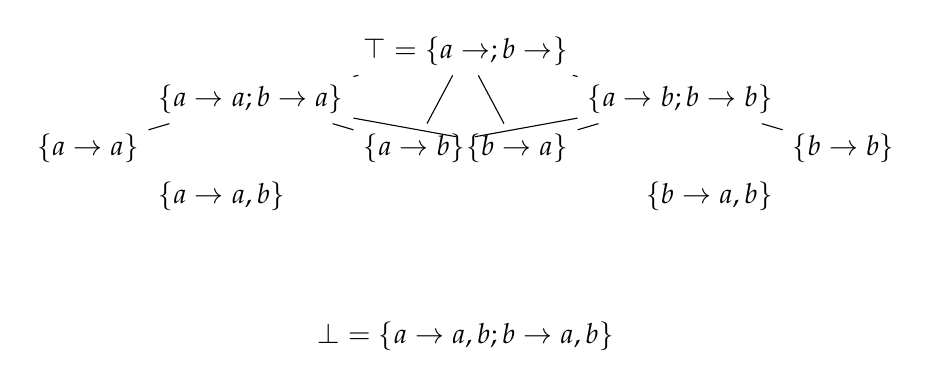
\begin{tikzpicture}[node distance=0em]
\node(top)                                        {$\top = \{a \rightarrow; b \rightarrow \}$};
\node(aa_ba)  [below left=\mydistance of top]     {$\{a \rightarrow a; b \rightarrow a\}$};
\node(ab_bb)  [below right=\mydistance of top]    {$\{a \rightarrow b; b \rightarrow b\}$};
\node(aa)     [below left=\mydistance of aa_ba]   {$\{a \rightarrow a\}$};
\node(ab)     [below right=\mydistance of aa_ba]  {$\{a \rightarrow b\}$};
\node(ba)     [below left=\mydistance of ab_bb]   {$\{b \rightarrow a\}$};
\node(bb)     [below right=\mydistance of ab_bb]  {$\{b \rightarrow b\}$};
\node(aab)    [below right=\mydistance of aa]     {$\{a \rightarrow a,b\}$};
\node(bab)    [below left=\mydistance of bb]      {$\{b \rightarrow a,b\}$};
\node(bottom) [below=3cm of top]  {$\bot = \{a \rightarrow a,b; b \rightarrow a,b\}$};
\draw (top) -- (aa_ba);
\draw (top) -- (ab_bb);
\draw (top) -- (ab);
\draw (top) -- (ba);
\draw (aa_ba) -- (aa);
\draw (aa_ba) -- (ab);
\draw (ab_bb) -- (ab);
\draw (ab_bb) -- (bb);
\draw (aa_ba) -- (ba);
\draw (ab_bb) -- (ba);
\end{tikzpicture}

  \caption{Graphical representation of a security lattice with the two principals: $a$ and $b$}
\end{figure}

\subsection{Implicit flows}
When assigning a value to a slot, possibly from another slot, it is an explicit flow.
In addition to explicit flows, it is also possible to have implicit flows throughout a program, due to conditional control structures (such as loops).
For whatever assignments we would do inside a block (or within a deeper block hierarchy) we need to take the predicates of these blocks into consideration.
This is done by adding the concept of \emph{program counter labels}, denoted \dlmpc.
For each scope we will have an implicit \dlmpc, depending on the surrounding predicates' labels.

\begin{example}{Implicit leak}\label{dlm:ex:implicit_leak}
  If we have the following program (each line commented with the current \dlmpc):
  \begin{lstlisting}[style=dlmc]
int {{a->z,y}} val = 0;   // $\mathcomment{\bot}$
int {{a->y}} cond = 1;    // $\mathcomment{\bot}$
if (cond) {
  val++;                  // $\mathcomment{\bot \sqcup \{a \rightarrow y\}}$
}
return val;               // $\mathcomment{\bot}$
  \end{lstlisting}
  In this example we would have an implicit leak of \dlmc{cond}, by way of \dlmc{val}.
  This is due to the assignment of \dlmc{val} inside of the \dlmc{if}-statement, as \dlmpc~ is increased to the join of the outer scope ($\bot$) and the label of the scope's predicate (\labelof{\dlmc{cond}}).
  For this program to pass \thetool, we would have to add a more strict policy to \dlmc{val}, so that it could match the policy of \dlmc{cond}.
\end{example}

\subsection{Authority and declassification}
In order to avoid mishaps by setting certain policies too lax, so that certain flows are permitted, we can temporarily set some policies to be more strict, and then only relax (\emph{declassify}) them when we really need to.
In order to do this, we need the concept of \emph{authority}.
At any point during running a program, it will have a \emph{true authority}, which is the maximal authority by which the program can carry out operations.
Whenever we call a function, we can do this with a certain authority, corresponding to running that method with the authority of a specific principal.
However, in order to take advantage of this given authority, we need to explicitly claim it.
This is done by using the \dlmactsfor\dlmc{(a, b)} function, where $a$ is the principal (typically the function itself) trying to obtain the authority of $b$.
Only after calling this function will we obtain the \emph{effective authority} to act for $b$, enabling us to carry out operations that would normally only be permissible for $b$ itself.

Inside the \dlmactsfor~ block, we now have the ability to carry out operations that normally would be permissible only to $b$ itself.
Most importantly, we can do declassification -- deliberately and explicitly relaxing the security policies in which $b$ is owner.
This is done by calling the \dlmdeclassify\dlmc{(v, l)} function, with a slot $v$ and a new label $l$ as inputs, returning the value $v$ relabeled to $l$.

The combination of these two concepts is especially useful when we have sensitive inputs to a method and want to carry out our calculations without the fear of neither explicit or implicit leakage.
This way we can keep our strict policies throughout the calculations of the method and only relax the label once we want to return the result.

\begin{example}{Temporarily restricting a label}
  Building on \cref{dlm:ex:implicit_leak}, we can set the label for \dlmc{val} to match that of \dlmc{cond}, and then only relax that label when we need to return \dlmc{val}, ensuring that we have the ability to do so:
  \begin{lstlisting}[style=dlmc]
int {{a->y}} val = 0;
int {{a->y}} cond = 1;
if (cond) {
  val++;
}
if_acts_for(this, a) {
  return declassify(x, {{a->y,z}});
}
return -1;
  \end{lstlisting}
  While we still leak some information about \dlmc{cond}, we do it explicitly.
\end{example}


\printbibliography[heading=bibintoc]
\label{bib:mybiblio}

\end{document}
